%
% This is the LaTeX template file for lecture notes for CS294-8,
% Computational Biology for Computer Scientists.  When preparing 
% LaTeX notes for this class, please use this template.
%
% To familiarize yourself with this template, the body contains
% some examples of its use.  Look them over.  Then you can
% run LaTeX on this file.  After you have LaTeXed this file then
% you can look over the result either by printing it out with
% dvips or using xdvi.
%
% This template is based on the template for Prof. Sinclair's CS 270.

\documentclass[twoside, 12pt]{article}
\usepackage{graphics}
\setlength{\oddsidemargin}{0.25 in}
\setlength{\evensidemargin}{-0.25 in}
\setlength{\topmargin}{-0.6 in}
\setlength{\textwidth}{6.5 in}
\setlength{\textheight}{8.5 in}
\setlength{\headsep}{0.75 in}
\setlength{\parindent}{0 in}
\setlength{\parskip}{0.1 in}


%
% The following commands set up the lecnum (lecture number)
% counter and make various numbering schemes work relative
% to the lecture number.
%
\newcounter{lecnum}
\renewcommand{\thepage}{\thelecnum-\arabic{page}}
\renewcommand{\thesection}{\thelecnum.\arabic{section}}
\renewcommand{\theequation}{\thelecnum.\arabic{equation}}
\renewcommand{\thefigure}{\thelecnum.\arabic{figure}}
\renewcommand{\thetable}{\thelecnum.\arabic{table}}

%
% The following macro is used to generate the header.
%
\newcommand{\lecture}[4]{
   \pagestyle{myheadings}
   \thispagestyle{plain}
   \newpage
   \setcounter{lecnum}{#1}
   \setcounter{page}{1}
   \noindent
   \begin{center}
   \framebox{
      \vbox{\vspace{2mm}
    \hbox to 6.28in { {\bf UGBA 141 Production and Operations Management
                        \hfill Spring 2022} }
       \vspace{4mm}
       \hbox to 6.28in { {\Large \hfill Cheatsheet #1: #2  \hfill} }
       \vspace{2mm}
       \hbox to 6.28in { {\it 
       Lecturer: #3 
       \hfill 
       GSI: #4} }
      \vspace{2mm}}
   }
   \end{center}
%  \markboth{Lecture #1: #2}{Lecture #1: #2}
%   {\bf Disclaimer}: {\it These notes have not been subjected to the
%   usual scrutiny reserved for formal publications.  They may be distributed
%   outside this class only with the permission of the Instructor.}
   \vspace*{4mm}
}

%
% Convention for citations is authors' initials followed by the year.
% For example, to cite a paper by Leighton and Maggs you would type
% \cite{LM89}, and to cite a paper by Strassen you would type \cite{S69}.
% (To avoid bibliography problems, for now we redefine the \cite command.)
% Also commands that create a suitable format for the reference list.
\renewcommand{\cite}[1]{[#1]}
\def\beginrefs{\begin{list}%
        {[\arabic{equation}]}{\usecounter{equation}
         \setlength{\leftmargin}{2.0truecm}\setlength{\labelsep}{0.4truecm}%
         \setlength{\labelwidth}{1.6truecm}}}
\def\endrefs{\end{list}}
\def\bibentry#1{\item[\hbox{[#1]}]}

%Use this command for a figure; it puts a figure in wherever you want it.
%usage: \fig{NUMBER}{SPACE-IN-INCHES}{CAPTION}
\newcommand{\fig}[3]{
			\vspace{#2}
			\begin{center}
			Figure \thelecnum.#1:~#3
			\end{center}
	}
% Use these for theorems, lemmas, proofs, etc.
\newtheorem{theorem}{Theorem}[lecnum]
\newtheorem{lemma}[theorem]{Lemma}
\newtheorem{proposition}[theorem]{Proposition}
\newtheorem{claim}[theorem]{Claim}
\newtheorem{corollary}[theorem]{Corollary}
\newtheorem{definition}[theorem]{Definition}
\newenvironment{proof}{{\bf Proof:}}{\hfill\rule{2mm}{2mm}}


% self added package
\usepackage{amsmath}
 \usepackage{graphicx}

% **** IF YOU WANT TO DEFINE ADDITIONAL MACROS FOR YOURSELF, PUT THEM HERE:

\begin{document}
%FILL IN THE RIGHT INFO.
%\lecture{**LECTURE-NUMBER**}{**DATE**}{**LECTURER**}{**SCRIBE**}
\lecture{4}{Supply Chain}{Park Sinchaisri}{Hansheng Jiang}
%\footnotetext{These notes are partially based on those of Nigel Mansell.}

% **** YOUR NOTES GO HERE:

% Some general latex examples and examples making use of the
% macros follow.  
%**** IN GENERAL, BE BRIEF. LONG SCRIBE NOTES, NO MATTER HOW WELL WRITTEN,
%**** ARE NEVER READ BY ANYBODY.

\begin{enumerate}
\item Let $Q$ denote the order quantity, and let $D$ denote the random demand with expectation/mean $\mu$.
\begin{itemize}
	\item Leftover inventory = $\max\{Q-D, 0\}$ = $Q- \min\{Q,D\}$
	\item Lost sales  = $\max\{D-Q, 0\}$ =  $D- \min\{Q,D\}$
	\item Sales  = $\min\{Q,D\}$
\end{itemize}

The following two fundamental equalities hold.
\[
\text{Expected lost sales + Expected sales } = \text{Expected demand } \mu
\]
\[
\text{Expected sales + Expected leftover inventory} = \text{Expected order quantity } Q.
\]

\item Read the ``Standard Normal Inventory/Loss Table''
\[
\text{Expected leftover inventory }= \text{Demand standard deviation } \sigma \times  I(z)
\]
where $z$ is the ratio of $(Q-\mu)/\sigma$, and $I()$ is the standard normal inventory function read from the table. 

\[
\text{Expected lost sales}= \text{Demand standard deviation } \sigma \times  L(z)
\]
where $z$ is the ratio of $(Q-\mu)/\sigma$, and $L()$ is the standard normal inventory function read from the table. 


\begin{figure}[!ht]
	\centering
	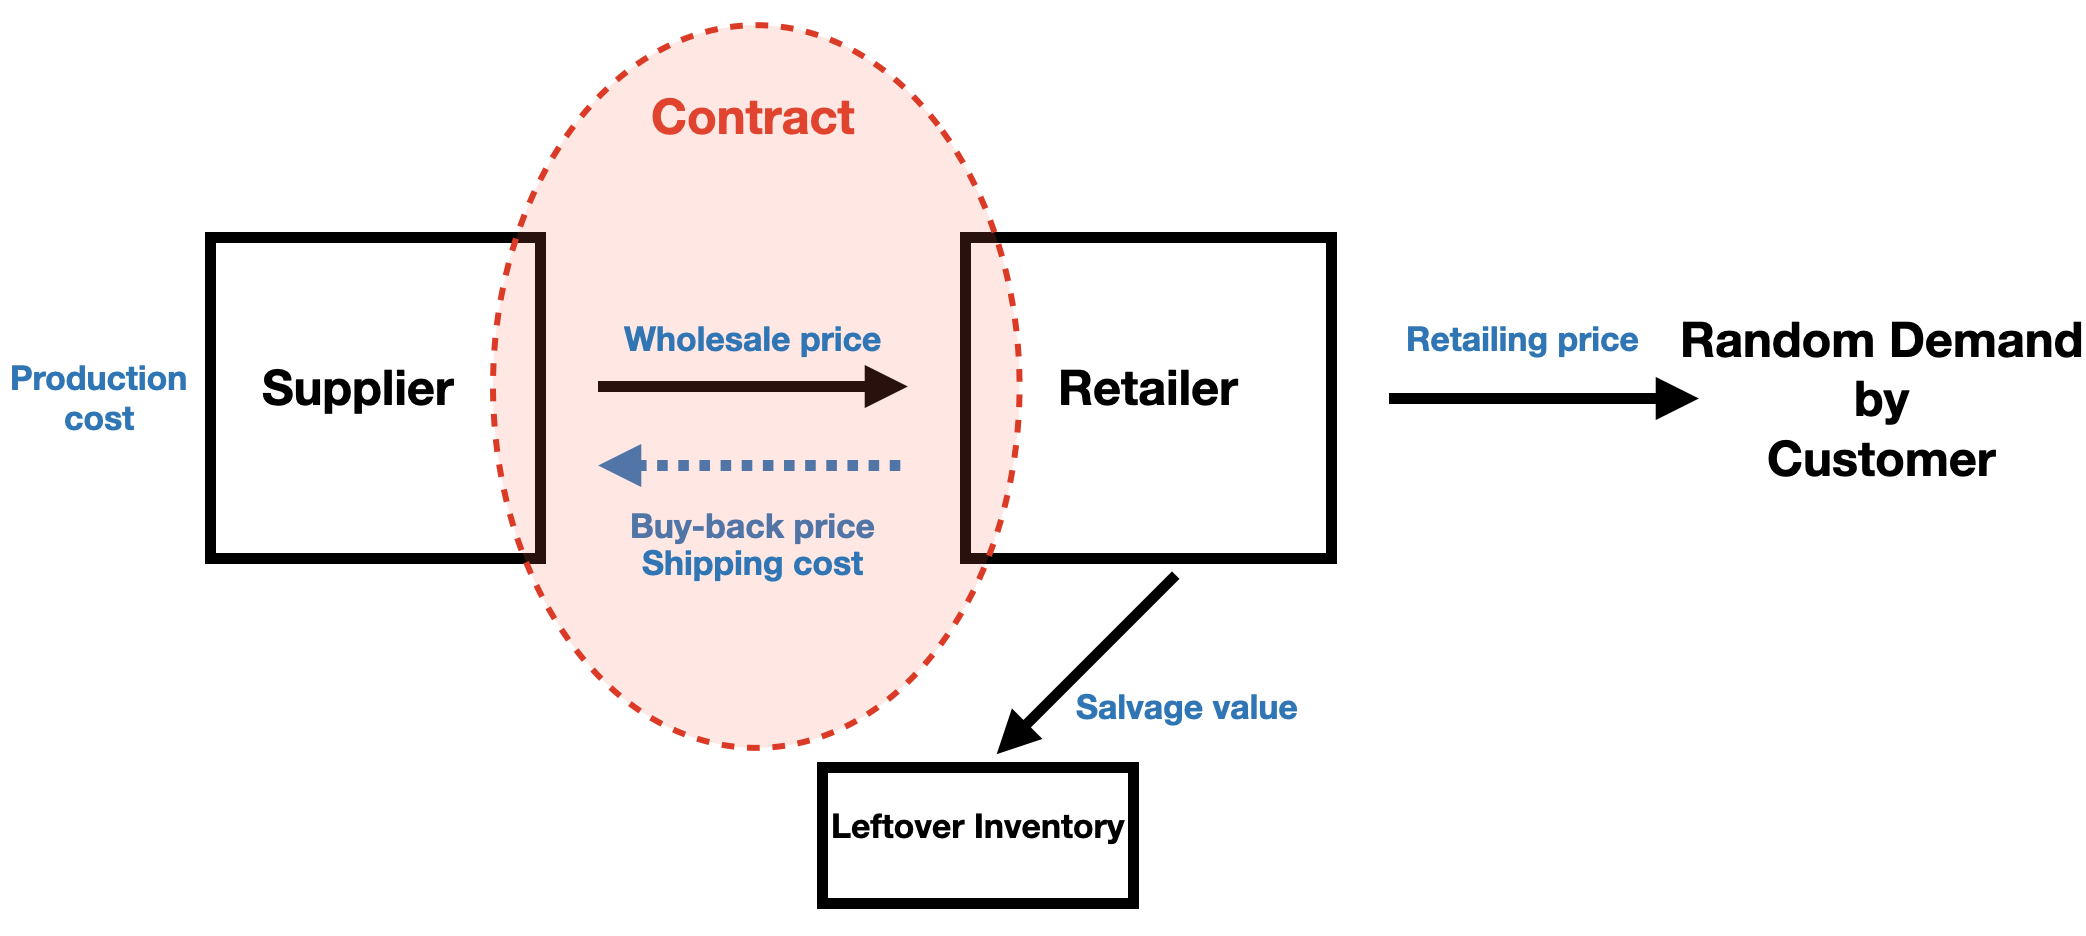
\includegraphics[width = 0.9\textwidth]{buyback-illustration}
	\caption{Illustration of Buy-back Contract}
\end{figure}

\item Expected profit of Newsvendor is
\[
G \times \text{Expected sales}  - L \times \text{Expected leftover inventory}
\]
where gain $G$ and loss $L$ need to be interpreted based on contexts by taking into consideration costs, prices, salvage value, and shipping costs whenever needed. Remember that alternatively, $G$ can be viewed as underage cost and $L$ can be viewed as overage cost.

\item Optimal Buy-back price  is equal to 
\[
\text{Shipping cost + Price } -    \frac{(\text{Price - Wholesale price})\times(\text{Price - Salvage value})}{\text{Price - Cost}},
\]
where `Price' refers to retailing price, and `Cost' refers to production cost. See the illustration in Figure~4.1.

\end{enumerate}















\section*{References}
\beginrefs


\bibentry{TC2006}{\sc C.~Terwiesch} and {\sc G.~Cachon}, 
  Matching supply with demand: An introduction to operations management (Chapter 14, 15, and 19), {McGraw-Hill~2006}
  

\endrefs


\end{document}





